\documentclass[a4paper,12pt]{article}
\usepackage{amsmath,amssymb,amsfonts,amsthm}
\usepackage{tikz}
\usepackage [utf8x] {inputenc}
\usepackage [T2A] {fontenc} 
\usepackage[russian]{babel}
\usepackage{cmap} 
\usepackage{ gensymb }
% Так ссылки в PDF будут активны
\usepackage[unicode]{hyperref}
\usepackage{ textcomp }
\usepackage{indentfirst}
\usepackage[version=3]{mhchem}

% вы сможете вставлять картинки командой \includegraphics[width=0.7\textwidth]{ИМЯ ФАЙЛА}
% получается подключать, как минимум, файлы .pdf, .jpg, .png.
\usepackage{graphicx}
% Если вы хотите явно указать поля:
\usepackage[margin=1in]{geometry}
% Или если вы хотите задать поля менее явно (чем больше DIV, тем больше места под текст):
% \usepackage[DIV=10]{typearea}

\usepackage{fancyhdr}

\newcommand{\bbR}{\mathbb R}%теперь вместо длинной команды \mathbb R (множество вещественных чисел) можно писать короткую запись \bbR. Вместо \bbR вы можете вписать любую строчку букв, которая начинается с '\'.
\newcommand{\eps}{\varepsilon}
\newcommand{\bbN}{\mathbb N}
\newcommand{\dif}{\mathrm{d}}

\newtheorem{Def}{Определение}


\pagestyle{fancy}
\makeatletter % сделать "@" "буквой", а не "спецсимволом" - можно использовать "служебные" команды, содержащие @ в названии
\fancyhead[L]{\footnotesize Лабораторные работы по общей физике}%Это будет написано вверху страницы слева
\fancyhead[R]{\footnotesize ФУПМ МФТИ}
%\fancyfoot[L]{\footnotesize \@author}%имя автора будет написано внизу страницы слева
\fancyfoot[R]{\thepage}%номер страницы —- внизу справа
\fancyfoot[C]{}%по центру внизу страницы пусто

\renewcommand{\maketitle}{%
	\noindent{\bfseries\scshape\large\@title\ \mdseries\upshape}\par
	\noindent {\large\itshape\@author}
	\vskip 2ex}
\makeatother
\def\dd#1#2{\frac{\partial#1}{\partial#2}}


\title{1.1. Фотоэффект}
\author{Хурсик Екатерина} 

\begin{document}	
\maketitle


\section{Цель работы}
    Экспериментально проверить уравнение Эйнштейна для фотоэффекта и определить
    постоянную Планка.
\section{Немного теории}
    \textit{Фотоэффект} -- испускание электронов веществом под действием электромагнитных
    излучений. Электроны, вылетающие из вещества при внешнем фотоэффекте,
    называются \textit{фотоэлектронами}, а электрический ток, образуемый ими при
    упорядоченном движении во внешнем электрическом поле, называется \textit{фототоком}.
    \begin{figure}[h!]
        \begin{center}
            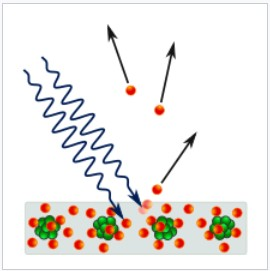
\includegraphics[width=0.3\linewidth]{2020-12-09-1.jpg}
            \caption{Схема фотоэффекта}
        \end{center}
    \end{figure}
    
    Фотоны (до столкновения с электроном фотокатода) обладают энергией
    $\hbar\omega$ и импульсом $\frac{\hbar\omega}{c}$. При столкновении фотона
    с электроном фотокатода энергия фотона полностью передаётся электрону.
    Для вылетающих электронов энергетический баланс можно описать уравнением
    \begin{equation}
        \hbar\omega=E_{max}+W,
    \end{equation}
    где $E_{max}$ - максимальная кинетическая энергия электрона после выхода из
    фотокатода, $W$ - работа выхода электрона из катода.

    Чтобы измерить энергии вылетевших фотоэлектронов вблизи фотокатода располагается
    второй электрод -- анод, на который подаётся потенциал ($V<0$ - задерживающий,
    $V>0$ - ускоряющий).

    \begin{figure}[h!]
        \begin{center}
            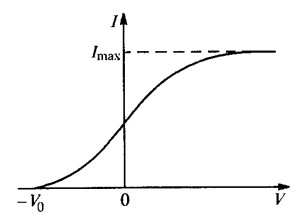
\includegraphics[width=0.5\linewidth]{2020-12-09-2.jpg}
            \caption{Зависимость фототока от напряжения на аноде фотоэлемента}
        \end{center}
    \end{figure}
    \pagebreak
    При достаточно больших ускоряющих напряжениях фототок
    достигает насыщения (рис.2): все испущенные электроны попадают на анод. При
    задерживающих потенциалах на анод попадают лишь электроны, обладающие
    достаточно большой кинетической энергией, в то время как медленно движущиеся
    электроны заворачиваются полем и возвращаются на катод. При некотором значении
    $V=-V_0$ -- \textit{потенциал запирания} -- даже наиболее быстрые электроны
    не могут достичь анода.

    Максимальная кинетическая энергия $E_{max}$ электронов связана с запирающим
    потенциалом $V_0$ соотношением
    \begin{equation}
        E_{max}=eV_0.
    \end{equation}
    Подставляя это соотношение в (1), мы получаем уравнение Эйнштейна для фотоэффекта:
    \begin{equation}
        eV_0=\hbar\omega-W
    \end{equation}

\section{Метод достижения цели}
    В работе изучается зависимость фототока из фотоэлемента от величины
    задерживающего потенциала $V$ для различных частот света $\omega$, лежащих в
    видимой области спектра. С целью экспериментальной проверки уравнения Эйнштейна
    определяются потенциалы запирания $V_0$ при разных частотах света и строится
    зависимость $V_0(\omega)$, которая, как это следует из (2), должна иметь вид
    \begin{equation}
        V_0(\omega)=\frac{(\hbar\omega-W)}{e}
    \end{equation}
    Потенциал запирания $V_0$ для любого катода линейно зависит от частоты света
    $\omega$. По наклону прямой на графике $V_0(\omega)$ (рис.3)
    \begin{figure}[h!]
        \begin{center}
            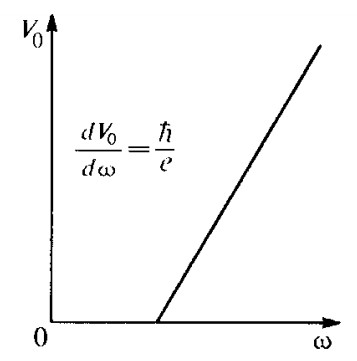
\includegraphics[width=0.4\linewidth]{2020-12-09-3.jpg}
            \caption{Зависимость запирающего потенциала от частоты света}
        \end{center}
    \end{figure}
    \pagebreak

    можно определить постоянную Планка:
    \begin{equation}
        \frac{dV_0}{d\omega}=\frac{\hbar}{e}.
    \end{equation}
\section{Вывод}
    Как показывает формула (5), угол наклона прямой $V_0(\omega)$ не зависит от рода
    вещества, но зависит величина фототока, работа выхода $W$ и форма кривой $I(V)$ (рис. 2).
\end{document}
